\documentclass[11pt,]{article}
\usepackage[left=1in,top=1in,right=1in,bottom=1in]{geometry}
\newcommand*{\authorfont}{\fontfamily{phv}\selectfont}
\usepackage[adobe-utopia]{mathdesign}


\usepackage[T1]{fontenc}
\usepackage[utf8]{inputenc}
\usepackage{inconsolata}

%\setmonofont{inconsolata}[Scale=0.5]

\usepackage{microtype}

\usepackage{geometry}
\geometry{a4paper, top=40mm, left=35mm, right=35mm, bottom=30mm}

\usepackage{fancyvrb} % Allows customization of verbatim environments
\fvset{fontsize=\normalsize} % The font size of all verbatim text can be changed here

\usepackage[all,defaultlines=3]{nowidow} % avoids widow and orphan sentences


\usepackage{abstract}
\renewcommand{\abstractname}{}    % clear the title
\renewcommand{\absnamepos}{empty} % originally center

\renewenvironment{abstract}
 {{%
    \setlength{\leftmargin}{0mm}
    \setlength{\rightmargin}{\leftmargin}%
  }%
  \relax}
 {\endlist}

\makeatletter
\def\@maketitle{%
  \newpage
%  \null
%  \vskip 2em%
%  \begin{center}%
  \let \footnote \thanks
    {\fontsize{18}{20}\selectfont\raggedright  \setlength{\parindent}{0pt} \@title \par}%
}
%\fi
\makeatother




\setcounter{secnumdepth}{0}

\usepackage{color}
\usepackage{fancyvrb}
\newcommand{\VerbBar}{|}
\newcommand{\VERB}{\Verb[commandchars=\\\{\}]}
\DefineVerbatimEnvironment{Highlighting}{Verbatim}{commandchars=\\\{\}}
% Add ',fontsize=\small' for more characters per line
\usepackage{framed}
\definecolor{shadecolor}{RGB}{248,248,248}
\newenvironment{Shaded}{\begin{snugshade}}{\end{snugshade}}
\newcommand{\KeywordTok}[1]{\textcolor[rgb]{0.13,0.29,0.53}{\textbf{#1}}}
\newcommand{\DataTypeTok}[1]{\textcolor[rgb]{0.13,0.29,0.53}{#1}}
\newcommand{\DecValTok}[1]{\textcolor[rgb]{0.00,0.00,0.81}{#1}}
\newcommand{\BaseNTok}[1]{\textcolor[rgb]{0.00,0.00,0.81}{#1}}
\newcommand{\FloatTok}[1]{\textcolor[rgb]{0.00,0.00,0.81}{#1}}
\newcommand{\ConstantTok}[1]{\textcolor[rgb]{0.00,0.00,0.00}{#1}}
\newcommand{\CharTok}[1]{\textcolor[rgb]{0.31,0.60,0.02}{#1}}
\newcommand{\SpecialCharTok}[1]{\textcolor[rgb]{0.00,0.00,0.00}{#1}}
\newcommand{\StringTok}[1]{\textcolor[rgb]{0.31,0.60,0.02}{#1}}
\newcommand{\VerbatimStringTok}[1]{\textcolor[rgb]{0.31,0.60,0.02}{#1}}
\newcommand{\SpecialStringTok}[1]{\textcolor[rgb]{0.31,0.60,0.02}{#1}}
\newcommand{\ImportTok}[1]{#1}
\newcommand{\CommentTok}[1]{\textcolor[rgb]{0.56,0.35,0.01}{\textit{#1}}}
\newcommand{\DocumentationTok}[1]{\textcolor[rgb]{0.56,0.35,0.01}{\textbf{\textit{#1}}}}
\newcommand{\AnnotationTok}[1]{\textcolor[rgb]{0.56,0.35,0.01}{\textbf{\textit{#1}}}}
\newcommand{\CommentVarTok}[1]{\textcolor[rgb]{0.56,0.35,0.01}{\textbf{\textit{#1}}}}
\newcommand{\OtherTok}[1]{\textcolor[rgb]{0.56,0.35,0.01}{#1}}
\newcommand{\FunctionTok}[1]{\textcolor[rgb]{0.00,0.00,0.00}{#1}}
\newcommand{\VariableTok}[1]{\textcolor[rgb]{0.00,0.00,0.00}{#1}}
\newcommand{\ControlFlowTok}[1]{\textcolor[rgb]{0.13,0.29,0.53}{\textbf{#1}}}
\newcommand{\OperatorTok}[1]{\textcolor[rgb]{0.81,0.36,0.00}{\textbf{#1}}}
\newcommand{\BuiltInTok}[1]{#1}
\newcommand{\ExtensionTok}[1]{#1}
\newcommand{\PreprocessorTok}[1]{\textcolor[rgb]{0.56,0.35,0.01}{\textit{#1}}}
\newcommand{\AttributeTok}[1]{\textcolor[rgb]{0.77,0.63,0.00}{#1}}
\newcommand{\RegionMarkerTok}[1]{#1}
\newcommand{\InformationTok}[1]{\textcolor[rgb]{0.56,0.35,0.01}{\textbf{\textit{#1}}}}
\newcommand{\WarningTok}[1]{\textcolor[rgb]{0.56,0.35,0.01}{\textbf{\textit{#1}}}}
\newcommand{\AlertTok}[1]{\textcolor[rgb]{0.94,0.16,0.16}{#1}}
\newcommand{\ErrorTok}[1]{\textcolor[rgb]{0.64,0.00,0.00}{\textbf{#1}}}
\newcommand{\NormalTok}[1]{#1}

\usepackage{graphicx,grffile}
\makeatletter
\def\maxwidth{\ifdim\Gin@nat@width>\linewidth\linewidth\else\Gin@nat@width\fi}
\def\maxheight{\ifdim\Gin@nat@height>\textheight\textheight\else\Gin@nat@height\fi}
\makeatother
% Scale images if necessary, so that they will not overflow the page
% margins by default, and it is still possible to overwrite the defaults
% using explicit options in \includegraphics[width, height, ...]{}
\setkeys{Gin}{width=\maxwidth,height=\maxheight,keepaspectratio}

\title{SITS - An R Package for Data Analysis and Machine Learning using
Satellite Image Time Series  }



\author{\Large Rolf Simoes\vspace{0.05in} \newline\normalsize\emph{National Institute for Space Reseach, INPE, Brazil}   \and \Large Gilberto Camara\vspace{0.05in} \newline\normalsize\emph{National Institute for Space Reseach, INPE, Brazil}   \and \Large Alexandre Iwata\vspace{0.05in} \newline\normalsize\emph{Institute for Applied Economics Research (IPEA), Brazil}   \and \Large Victor Maus\vspace{0.05in} \newline\normalsize\emph{International Institute for Applied System Analysis (IIASA)}  }


\date{}

\usepackage{titlesec}

\titleformat*{\section}{\normalsize\bfseries}
\titleformat*{\subsection}{\normalsize\itshape}
\titleformat*{\subsubsection}{\normalsize\itshape}
\titleformat*{\paragraph}{\normalsize\itshape}
\titleformat*{\subparagraph}{\normalsize\itshape}


\usepackage{natbib}
\bibliographystyle{agsm}
\usepackage[strings]{underscore} % protect underscores in most circumstances



\newtheorem{hypothesis}{Hypothesis}
\usepackage{setspace}

\makeatletter
\@ifpackageloaded{hyperref}{}{%
\ifxetex
  \PassOptionsToPackage{hyphens}{url}\usepackage[setpagesize=false, % page size defined by xetex
              unicode=false, % unicode breaks when used with xetex
              xetex]{hyperref}
\else
  \PassOptionsToPackage{hyphens}{url}\usepackage[unicode=true]{hyperref}
\fi
}

\@ifpackageloaded{color}{
    \PassOptionsToPackage{usenames,dvipsnames}{color}
}{%
    \usepackage[usenames,dvipsnames]{color}
}
\makeatother
\hypersetup{breaklinks=true,
            bookmarks=true,
            pdfauthor={Rolf Simoes (National Institute for Space Reseach, INPE, Brazil) and Gilberto Camara (National Institute for Space Reseach, INPE, Brazil) and Alexandre Iwata (Institute for Applied Economics Research (IPEA), Brazil) and Victor Maus (International Institute for Applied System Analysis (IIASA))},
             pdfkeywords = {},
            pdftitle={SITS - An R Package for Data Analysis and Machine Learning using
Satellite Image Time Series},
            colorlinks=true,
            citecolor=blue,
            urlcolor=blue,
            linkcolor=magenta,
            pdfborder={0 0 0}}
\urlstyle{same}  % don't use monospace font for urls

% set default figure placement to htbp
\makeatletter
\def\fps@figure{htbp}
\makeatother



% add tightlist ----------
\providecommand{\tightlist}{%
\setlength{\itemsep}{0pt}\setlength{\parskip}{12pt}}

\begin{document}

% \pagenumbering{arabic}% resets `page` counter to 1
%
% \maketitle

{% \usefont{T1}{pnc}{m}{n}
\setlength{\parindent}{0pt}
\thispagestyle{plain}
{\fontsize{18}{20}\selectfont\raggedright
\maketitle  % title \par

}

{
   \vskip 13.5pt\relax \normalsize\fontsize{11}{12}
\textbf{\authorfont Rolf Simoes} \hskip 15pt \emph{\small National Institute for Space Reseach, INPE, Brazil}   \par \textbf{\authorfont Gilberto Camara} \hskip 15pt \emph{\small National Institute for Space Reseach, INPE, Brazil}   \par \textbf{\authorfont Alexandre Iwata} \hskip 15pt \emph{\small Institute for Applied Economics Research (IPEA), Brazil}   \par \textbf{\authorfont Victor Maus} \hskip 15pt \emph{\small International Institute for Applied System Analysis (IIASA)}   

}

}








\begin{abstract}

    \hbox{\vrule height .2pt width 39.14pc}

    \vskip 8.5pt % \small

\noindent Using time series derived from big Earth Observation data sets is one of
the leading research trends in Land Use Science and Remote Sensing. One
of the more promising uses of satellite time series is its application
for classification of land use and land cover, since our growing demand
for natural resources has caused major environmental impacts. The SITS
package provides support on how to use statistical learning techniques
with image time series. These methods include linear and quadratic
discrimination analysis, support vector machines, random forests and
neural networks.


    \hbox{\vrule height .2pt width 39.14pc}


\end{abstract}


\vskip 6.5pt

\setlength{\parskip}{6pt}
%\renewcommand{\baselinestretch}{15pt}
\noindent  \section{Introduction}\label{introduction}

Earth observation satellites provide a continuous and consistent set of
information about the Earth's land and oceans. Most space agencies have
adopted an open data policy, making unprecedented amounts of satellite
data available for research and operational use. This data deluge has
brought about a major challenge:
\textit{How to design and build technologies that allow the Earth observation community to analyse big data sets?}

The approach taken in the current package is to develop data analysis
methods that work with satellite image time series (SITS). The time
series are obtained by taking calibrated and comparable measures of the
same location in Earth at different times. These measures can be
obtained by a single sensor (e.g., MODIS) or by combining different
sensores (e.g., LANDSAT-8 and SENTINEL-2). If obtained by frequent
revisits, the temporal resolution of these data sets can capture the
most important land use changes.

Time series of remote sensing data show that land cover changes do not
always occur in a progressive and gradual way, but they may also show
periods of rapid and abrupt change followed either by a quick recovery
\citep{Lambin2003}. Analyses of multiyear time series of land surface
attributes, their fine-scale spatial pattern, and their seasonal
evolution leads to a broader view of land-cover change. Satellite image
time series have already been applied to applications such as mapping
for detecting forest disturbance \citep{Kennedy2010}, ecology dynamics
\citep{Pasquarella2016}, agricultural intensification
\citep{Galford2008} and its impacts on deforestation \citep{Arvor2012}.

The SITS package provides support on how to use statistical learning
techniques with image time series. In a broad sense, statistical
learning refers to a class of algorithms for classification and
regression analysis \citep{Hastie2009}. These methods include linear and
quadratic discrimination analysis, support vector machines, random
forests and neural networks. In a typical classification problem, we
have measures that capture class attributes. Based on these measures,
referred as training data, one's task is to select a predictive model
that allows inferring classes of a larger data set.

Current approaches to image time series analysis still use limited
number of attributes. A common approach is deriving a small set of
phenological parameters from vegetation indexes, like beginning, peak,
and length of growing season \citep{Brown2013} \citep{Kastens2017}
\citep{Estel2015} \citep{Pelletier2016}. These phenological parameters
are then fed in specialised classifiers such as TIMESAT
\citep{Jonsson2004}. These approaches do not use the power of advanced
statistical learning techniques to work on high-dimensional spaces and
with big training data sets \citep{James2013}.

The SITS package uses the full depth of satellite image time series to
create larger dimensional spaces. We tested different methods of
extracting attributes from time series data, including those reported by
\citet{Pelletier2016} and \citet{Kastens2017}. Our conclusion is that
part of the information in raw time series is lost after filtering or
statistical approximation. Thus, the method we developed has a deceptive
simplicity:
\emph{use all the data available in the time series samples}. The idea
is to have as many temporal attributes as possible, increasing the
dimension of the classification space. Our experiments found out that
modern statistical models such as support vector machines, and random
forests perform better in high-dimensional spaces than in lower
dimensional ones.

In what follows, we describe the main characteristics of the SITS
package. The first part describes the basic data structures used in SITS
and the tools used for visualisation and data exploration. Then we show
how to do data acquision from external sources, with an emphasis on the
WTSS (``web time series service''). The next sections describe filtering
and clustering techniques. We then discuss machine learning techiques
for SITS data and how to apply them to image time series. Finally, we
present validation methods.

\section{Data Handling and Visualisation Basics in
SITS}\label{data-handling-and-visualisation-basics-in-sits}

The basic data unit in the sits package is the SITS tibble, which is a
way of organizing a set of time series data with associated spatial
information. In R, a ``tibble'' differs from the traditional data frame,
insofar as a tibble can contain lists embedded as column arguments.
Tibbles are part of the ``tidyverse'', a collection of R package
designed to work together in data manipulation. The ``tidyverse''
includes packages such as ``ggplot2'', ``dplyr'' and ``purrr''
\citep{Wickham2017}. The ``SITS'' package makes extensive use of the
``tidyverse''.

For a better explanation of how the ``SITS tibble'' works, we will read
a data set containing 2,115 labelled samples of land cover in Mato
Grosso state of Brazil. This state has 903,357 km\textsuperscript{2} of
extension, being the third largest state of Brazil. It includes three of
Brazil's biomes: Amazonia, Cerrado and Pantanal. It is the most
important agricultural frontier of Brazil and is Brazil's largest
producer of soybeans, corn and cotton.

The samples contain time series extracted from the MODIS MOD13Q1 product
from NASA from 2001 to 2016, provided every 16 days at 250-meter spatial
resolution in the Sinusoidal projection. Based on ground surveys and
high resolution imagery, we selected 2,115 samples of nine classes:
forest, cerrado, pasture, soybean-fallow, fallow-cotton, soybean-cotton,
soybean-corn, (8) soybean-millet, soybean-sunflower. Crop and pasture
ground data was collected by researchers Alexandre Coutinho, Julio
Esquerdo and Joao Antunes from the Brazilian Agricultural Research
Agency (EMBRAPA) through farmer interviews in October 2009 and in
October 2013. Samples for cerrado and forest classes were provided by
Rodrigo Bergotti from INPE. Ground samples for soybean-fallow class were
provided by Damien Arvor\citep{Arvor2012}.

\begin{Shaded}
\begin{Highlighting}[]
\CommentTok{# retrieve a set of samples from an RDS file}
\NormalTok{samples.tb <-}\StringTok{ }\KeywordTok{readRDS}\NormalTok{(}\KeywordTok{system.file}\NormalTok{(}\StringTok{"extdata/time_series/embrapa_mt.rds"}\NormalTok{, }
                                     \DataTypeTok{package =} \StringTok{"sits"}\NormalTok{))}
\NormalTok{samples.tb}
\end{Highlighting}
\end{Shaded}

\begin{verbatim}
## # A tibble: 2,115 x 7
##    longitude latitude start_date   end_date   label    coverage
##        <dbl>    <dbl>     <date>     <date>   <chr>       <chr>
##  1  -55.1852 -10.8378 2013-09-14 2014-08-29 Pasture mod13q1_512
##  2  -57.7940  -9.7573 2006-09-14 2007-08-29 Pasture mod13q1_512
##  3  -51.9412 -13.4198 2014-09-14 2015-08-29 Pasture mod13q1_512
##  4  -55.9643 -10.0621 2005-09-14 2006-08-29 Pasture mod13q1_512
##  5  -54.5540 -10.3749 2013-09-14 2014-08-29 Pasture mod13q1_512
##  6  -52.4572 -10.9512 2013-09-14 2014-08-29 Pasture mod13q1_512
##  7  -52.1443 -13.9981 2013-09-14 2014-08-29 Pasture mod13q1_512
##  8  -57.6907 -13.3382 2015-09-14 2016-08-28 Pasture mod13q1_512
##  9  -54.7034 -16.4265 2015-09-14 2016-08-28 Pasture mod13q1_512
## 10  -53.6543 -15.7155 2014-09-14 2015-08-29 Pasture mod13q1_512
## # ... with 2,105 more rows, and 1 more variables: time_series <list>
\end{verbatim}

The ``SITS tibble'' contains data and metadata. The first six columns
contain the metadata: spatial and temporal location, label assigned to
the sample, and coverage from where the data has been extracted. The
spatial location is given in longitude and latitude coordinates for the
``WGS84'' ellipsoid. For example, the first sample has been labelled
``Pasture'', at location (-55.1852, -10.8387), and is considered valid
for the period (2013-09-14, 2014-08-29). Informing the dates where the
label is valid is crucial for correct classification. In this case, the
researchers involved in labelling the samples chose to use the
agricultural calendar in Brazil, where the spring crop is planted in the
months of September and October, and the autmun crop is planted in the
months of February and March. For other applications and other
countries, the relevant dates will most likely be different from those
used in the example.

The SITS tibble also contains the time series data for each
spatiotemporal location. The timeseries data is also organized as a
tibble, with a column with the dates and the other columns with the
values for each spectral band.

\begin{Shaded}
\begin{Highlighting}[]
\CommentTok{#print the first time series}
\NormalTok{samples.tb[}\DecValTok{1}\NormalTok{,]}\OperatorTok{$}\NormalTok{time_series}
\end{Highlighting}
\end{Shaded}

\begin{verbatim}
## [[1]]
## # A tibble: 23 x 7
##         Index   ndvi    evi    nir    mir   blue    red
##  *     <date>  <dbl>  <dbl>  <dbl>  <dbl>  <dbl>  <dbl>
##  1 2013-09-14 0.4245 0.2800 0.2879 0.2439 0.0605 0.1163
##  2 2013-09-30 0.4673 0.2642 0.2570 0.1672 0.0357 0.0933
##  3 2013-10-16 0.5039 0.2993 0.2659 0.2019 0.0405 0.0877
##  4 2013-11-01 0.6489 0.4071 0.2762 0.1026 0.0266 0.0588
##  5 2013-11-17 0.7956 0.6692 0.4552 0.0875 0.0271 0.0518
##  6 2013-12-03 0.7248 0.5400 0.3661 0.0799 0.0516 0.0584
##  7 2013-12-19 0.7971 0.5574 0.3490 0.0478 0.0171 0.0394
##  8 2014-01-01 0.8049 0.7228 0.5255 0.1030 0.0327 0.0568
##  9 2014-01-17 0.7364 0.6867 0.5165 0.1449 0.0629 0.0784
## 10 2014-02-02 0.7870 0.7342 0.5320 0.1323 0.0452 0.0634
## # ... with 13 more rows
\end{verbatim}

The SITS package provides functions for data manipulation and displaying
information of a SITS tibble. For example, the function is
\texttt{sits\_bands} that lists the available bands.

\begin{Shaded}
\begin{Highlighting}[]
\KeywordTok{sits_bands}\NormalTok{ (samples.tb)}
\end{Highlighting}
\end{Shaded}

\begin{verbatim}
## [1] "ndvi" "evi"  "nir"  "mir"  "blue" "red"
\end{verbatim}

Another useful command is \texttt{sits\_labels} that shows the labels of
the sample set and their frequencies.

\begin{Shaded}
\begin{Highlighting}[]
\KeywordTok{sits_labels}\NormalTok{ (samples.tb)}
\end{Highlighting}
\end{Shaded}

\begin{verbatim}
## # A tibble: 9 x 3
##           label count       freq
##           <chr> <int>      <dbl>
## 1       Cerrado   400 0.18912530
## 2 Fallow_Cotton    34 0.01607565
## 3        Forest   138 0.06524823
## 4       Pasture   370 0.17494090
## 5      Soy_Corn   398 0.18817967
## 6    Soy_Cotton   399 0.18865248
## 7    Soy_Fallow    88 0.04160757
## 8    Soy_Millet   235 0.11111111
## 9 Soy_Sunflower    53 0.02505910
\end{verbatim}

In many cases, it is useful to relabel the data set. For examples, there
may be situations when one wants to use a smaller set of labels, since
samples in one label on the original set may not be distinguishable for
samples with other labels. We then should use the \texttt{sits\_relabel}
function. This function requires a conversion list, as shown in the
example below.

\begin{Shaded}
\begin{Highlighting}[]
\CommentTok{# a list for relabelling the samples}
\NormalTok{new_labels <-}\StringTok{ }\KeywordTok{list}\NormalTok{(}\StringTok{"Cerrado"}\NormalTok{       =}\StringTok{ "Savanna"}\NormalTok{, }
                   \StringTok{"Pasture"}\NormalTok{       =}\StringTok{ "Grasslands"}\NormalTok{, }
                   \StringTok{"Soy_Corn"}\NormalTok{      =}\StringTok{ "Double_Cropping"}\NormalTok{,}
                   \StringTok{"Soy_Cotton"}\NormalTok{    =}\StringTok{ "Double_Cropping"}\NormalTok{,}
                   \StringTok{"Soy_Sunflower"}\NormalTok{ =}\StringTok{ "Double_Cropping"}\NormalTok{,}
                   \StringTok{"Soy_Fallow"}\NormalTok{    =}\StringTok{ "Single_Cropping"}\NormalTok{,}
                   \StringTok{"Soy_Millet"}\NormalTok{    =}\StringTok{ "Single_Cropping"}\NormalTok{,}
                   \StringTok{"Fallow_Cotton"}\NormalTok{ =}\StringTok{ "Single_Cropping"}\NormalTok{)}
\CommentTok{# apply the sits_relabel function}
\NormalTok{samples2.tb <-}\StringTok{ }\KeywordTok{sits_relabel}\NormalTok{(samples.tb, new_labels)}
\CommentTok{# view the result}
\KeywordTok{sits_labels}\NormalTok{(samples2.tb)}
\end{Highlighting}
\end{Shaded}

\begin{verbatim}
## # A tibble: 5 x 3
##             label count       freq
##             <chr> <int>      <dbl>
## 1 Double_Cropping   850 0.40189125
## 2          Forest   138 0.06524823
## 3      Grasslands   370 0.17494090
## 4         Savanna   400 0.18912530
## 5 Single_Cropping   357 0.16879433
\end{verbatim}

Given that we have used the tibble data format for the metadata and and
the embedded time series, one can use the functions of the
\texttt{dplyr}, \texttt{tidyr} and \texttt{purrr} packages of the
``tidyverse'' \citep{Wickham2017} to process the data. For example, the
following example uses the \texttt{sits\_select} function to get a
subset of the sample data set with two bands (``ndvi'' and ``evi'') and
then uses the \texttt{dplyr::filter} function to select the samples
labelled either as ``Cerrado'' or ``Pasture''. We can then use the
\texttt{sits\_plot} function to display the time series. Given a small
number of samples to display, the \texttt{sits\_plot} function tries to
group as many spatial locations together. In the following example, the
first 15 samples of the ``Cerrado'' class all refer to the same spatial
location in consecutive times. For this reason, these samples are
plotted together.

\begin{Shaded}
\begin{Highlighting}[]
\CommentTok{# select the "ndvi" bands}
\NormalTok{samples_ndvi.tb <-}\StringTok{ }\KeywordTok{sits_select}\NormalTok{(samples.tb, }\DataTypeTok{bands =} \KeywordTok{c}\NormalTok{(}\StringTok{"ndvi"}\NormalTok{))}
\CommentTok{# select only the samples with the cerrado label}
\NormalTok{samples_cerrado.tb <-}\StringTok{ }\NormalTok{dplyr}\OperatorTok{::}\KeywordTok{filter}\NormalTok{ (samples_ndvi.tb, label }\OperatorTok{==}\StringTok{ "Cerrado"}\NormalTok{)}
\CommentTok{# plot the first 15 samples (different dates for the same points)}
\KeywordTok{sits_plot}\NormalTok{ (samples_cerrado.tb[}\DecValTok{1}\OperatorTok{:}\DecValTok{15}\NormalTok{,])}
\end{Highlighting}
\end{Shaded}

\begin{center}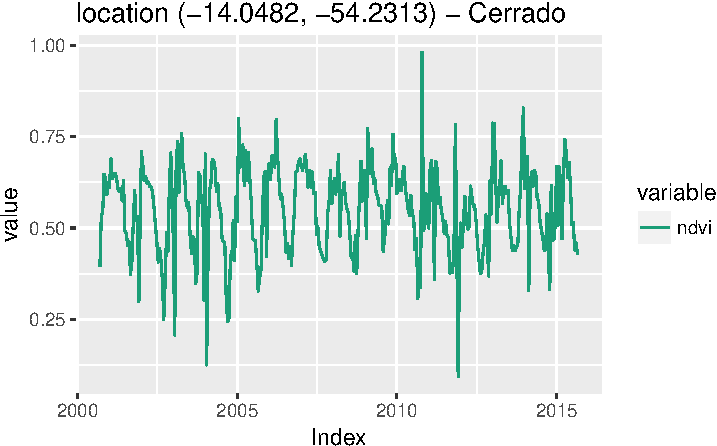
\includegraphics{sits_description_files/figure-latex/unnamed-chunk-10-1} \end{center}

For a large number of samples, where the amount of individual plots
would be substantial, the default visualisation combines all samples
together in a single temporal interval (even if they are valid for
different years). Therefore, all samples of the same band and the same
label are aligned to a common interval. This plot is useful to show the
spread of values for the time series of each band. The strong red line
in the plot shows the median of the values, and the two orange lines are
the first and third interquartile ranges. The \texttt{sits\_plot}
function has different ways of working. Please refer to the
documentation for more details.

\begin{Shaded}
\begin{Highlighting}[]
\CommentTok{# plot all cerrado samples together (shows the distribution)}
\KeywordTok{sits_plot}\NormalTok{ (samples_cerrado.tb)}
\end{Highlighting}
\end{Shaded}

\begin{center}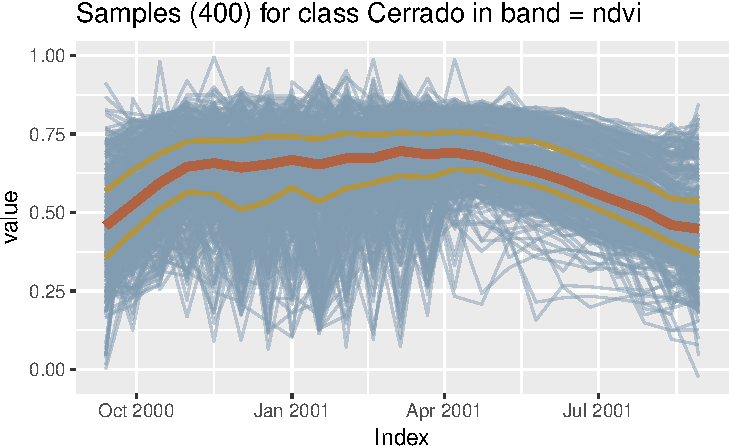
\includegraphics{sits_description_files/figure-latex/unnamed-chunk-11-1} \end{center}

\section{Importing data into SITS}\label{importing-data-into-sits}

The SITS package allows different methods of data input, including: (a)
obtain data from a WTSS (Web Series Time Service); (b) read data stored
in a time series in the ZOO format \citep{Zeileis2005}; (c) read a time
series from a RasterBrick \citep{Hijmans2015}. This section describes
options (a) and (b). Option (c) will be described in the section were we
describe raster processing. The WTSS service is a light-weight service,
designed to retrieve time series for selected locations and periods
\citep{Vinhas2016}. This service has been implemented by the research
team of the National Institute for Space Research to allow remote access
to time series data. To access the service, the user needs to provide a
URL that points to the WTSS server location and use the function
\texttt{sits\_infoWTSS} that provides information on the coverages
available on the server.

\begin{Shaded}
\begin{Highlighting}[]
\NormalTok{URL <-}\StringTok{ "http://www.dpi.inpe.br/tws/wtss"}
\NormalTok{wtss_inpe <-}\StringTok{ }\KeywordTok{sits_infoWTSS}\NormalTok{(URL)}
\end{Highlighting}
\end{Shaded}

\begin{verbatim}
## -----------------------------------------------------------
## The WTSS server URL is http://www.dpi.inpe.br/tws/wtss
## Available coverages: 
## MOD13Q1
## itobi
## merge
## mod13q1_512
## ------------------------------------------------------------
\end{verbatim}

After finding out which coverages are available at the WTSS service, one
may request specific information on each coverage by using the function
\texttt{sits\_coverageWTSS} which lists the contents of the data set,
including source, bands, spatial extent and resolution, time range, and
temporal resolution. This information is then stored in a tibble for
later use.

\begin{Shaded}
\begin{Highlighting}[]
\CommentTok{# get information about a specific coverage}
\NormalTok{coverage.tb <-}\StringTok{ }\KeywordTok{sits_coverageWTSS}\NormalTok{(URL,}\StringTok{"mod13q1_512"}\NormalTok{)}
\end{Highlighting}
\end{Shaded}

\begin{verbatim}
## ----------------------------------------------------------------------------------
## Coverage: mod13q1_512
## Description: Vegetation Indices 16-Day L3 Global 250m
## Source: https://lpdaac.usgs.gov/dataset_discovery/modis/modis_products_table/mod13q1
## Bands: 
##   name                            description
## 1 ndvi                      250m 16 days NDVI
## 2  evi                       250m 16 days EVI
## 3  red  250m 16 days red reflectance (Band 1)
## 4  nir  250m 16 days NIR reflectance (Band 2)
## 5 blue 250m 16 days blue reflectance (Band 3)
## 6  mir  250m 16 days MIR reflectance (Band 7)
## 
## Spatial extent: (-180, -90) - (180, 90)
## Spatial resolution: (0.00208334, 0.00208334)
## Projection CRS: +proj=longlat +ellps=WGS84 +datum=WGS84 +no_defs
## Time range: 2000-02-18 to 2017-02-18
## Temporal resolution: 16 days 
## ----------------------------------------------------------------------------------
\end{verbatim}

The user can then request one or more points using the
\texttt{sits\_getdata} function. This function provides a general means
of access to image time series. In it simplest fashion, the user
provides the latitude and longitude of the desired location, the URL of
the WTSS services, the coverage name, the bands, and the start date and
end date of the time series. If the start and end dates are not
provided, all of the samples are retrived. The result is a SITS tibble
that can be visualised using \texttt{sits\_plot}.

\begin{Shaded}
\begin{Highlighting}[]
\CommentTok{# a point in the transition forest pasture in Northern MT}
\NormalTok{long <-}\StringTok{ }\OperatorTok{-}\FloatTok{55.57320}
\NormalTok{lat <-}\StringTok{ }\OperatorTok{-}\FloatTok{11.50566}
\CommentTok{# obtain a time series from the WTSS server for this point}
\NormalTok{series.tb <-}\StringTok{ }\KeywordTok{sits_getdata}\NormalTok{(}\DataTypeTok{longitude =}\NormalTok{ long, }\DataTypeTok{latitude =}\NormalTok{ lat, }\DataTypeTok{URL =}\NormalTok{ URL, }
                          \DataTypeTok{coverage =} \StringTok{"mod13q1_512"}\NormalTok{, }\DataTypeTok{bands =} \KeywordTok{c}\NormalTok{(}\StringTok{"ndvi"}\NormalTok{, }\StringTok{"evi"}\NormalTok{),}
                          \DataTypeTok{start_date =} \StringTok{"2001-01-01"}\NormalTok{, }\DataTypeTok{end_date =} \StringTok{"2016-12-31"}\NormalTok{)}
\CommentTok{# plot the series}
\KeywordTok{sits_plot}\NormalTok{ (series.tb)}
\end{Highlighting}
\end{Shaded}

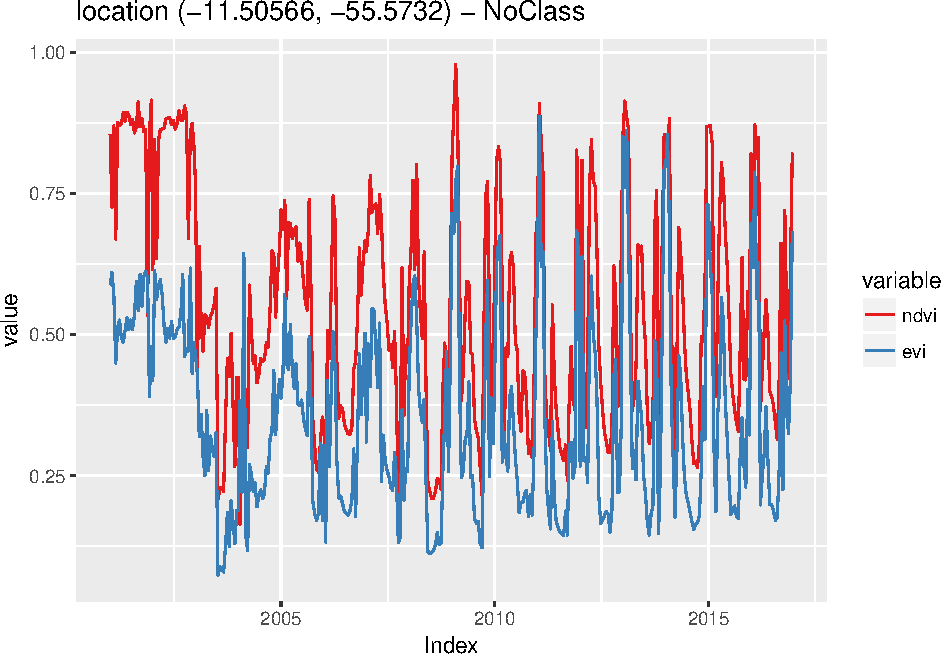
\includegraphics{sits_description_files/figure-latex/unnamed-chunk-14-1.pdf}
\newpage
\singlespacing
\bibliography{references-sits.bib}
\end{document}
